% Horizontal bar chart: success rate per QUALITY metric across 9 runs
% Usage: % Horizontal bar chart: success rate per QUALITY metric across 9 runs
% Usage: % Horizontal bar chart: success rate per QUALITY metric across 9 runs
% Usage: % Horizontal bar chart: success rate per QUALITY metric across 9 runs
% Usage: \input{generated/variability-quality.tex}

\definecolor{cQual}{HTML}{548235}

\begin{figure}[H]
\centering
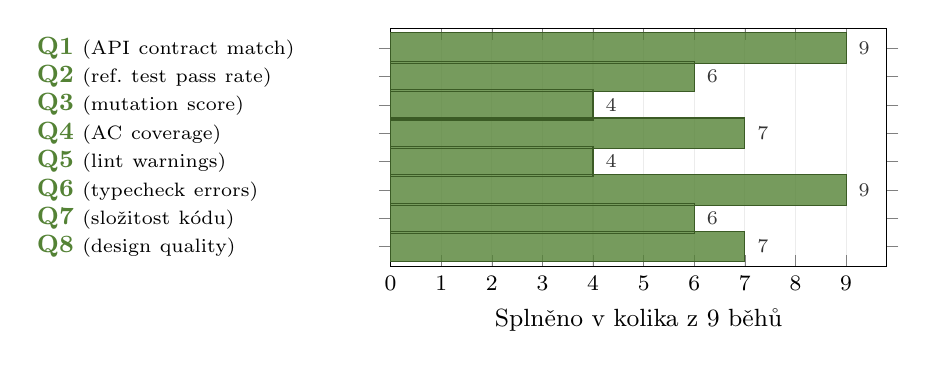
\begin{tikzpicture}
\begin{axis}[
    xbar,
    width=0.65\textwidth,
    height=0.38\textwidth,
    xlabel={Splněno v~kolika z~9 běhů},
    xmin=0, xmax=9.8,
    xtick={0,1,2,3,4,5,6,7,8,9},
    ymin=0.3, ymax=8.7,
    ytick={1,2,3,4,5,6,7,8},
    yticklabels={
        {\textcolor{cQual}{\textbf{Q8}} {\scriptsize(design quality)}},
        {\textcolor{cQual}{\textbf{Q7}} {\scriptsize(složitost kódu)}},
        {\textcolor{cQual}{\textbf{Q6}} {\scriptsize(typecheck errors)}},
        {\textcolor{cQual}{\textbf{Q5}} {\scriptsize(lint warnings)}},
        {\textcolor{cQual}{\textbf{Q4}} {\scriptsize(AC coverage)}},
        {\textcolor{cQual}{\textbf{Q3}} {\scriptsize(mutation score)}},
        {\textcolor{cQual}{\textbf{Q2}} {\scriptsize(ref.\ test pass rate)}},
        {\textcolor{cQual}{\textbf{Q1}} {\scriptsize(API contract match)}}
    },
    yticklabel style={font=\small, anchor=east, text width=12em, align=left},
    xticklabel style={font=\footnotesize},
    xlabel style={font=\small},
    bar width=11pt,
    nodes near coords,
    nodes near coords style={font=\scriptsize, anchor=west, xshift=1pt},
    xmajorgrids=true,
    ymajorgrids=false,
    grid style={gray!15},
    clip=false,
]

\addplot[fill=cQual, draw=cQual!70!black, fill opacity=0.8] coordinates {
    (7,1)   % Q8 >=2/3: 7/9
    (6,2)   % Q7 <=1: 6/9
    (9,3)   % Q6 =0: 9/9
    (4,4)   % Q5 <=1: 4/9
    (7,5)   % Q4 >=24: 7/9
    (4,6)   % Q3 >=70%: 4/7 (2 N/A)
    (6,7)   % Q2 >=37: 6/9
    (9,8)   % Q1 match: 9/9
};

\end{axis}
\end{tikzpicture}
\caption{Míra splnění exit kritérií \mgrp{Q} napříč devíti běhy.
\acs{Q1} a~\acs{Q6} byly splněny ve všech bězích;
\acs{Q3} a~\acs{Q5} nejméně často.
\acs{Q3} počítáno ze~7 běhů (2~bez dat).
Metriky efektivity (E1--E3) nemají exit kritérium a~nejsou zahrnuty.}
\label{fig:variability-quality}
\end{figure}


\definecolor{cQual}{HTML}{548235}

\begin{figure}[H]
\centering
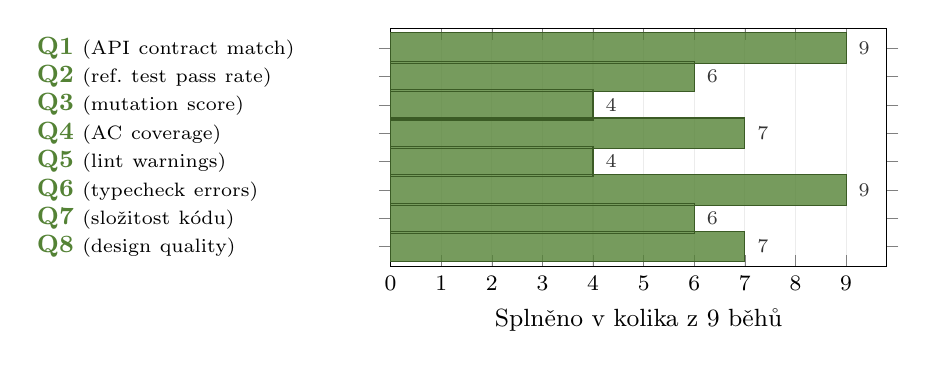
\begin{tikzpicture}
\begin{axis}[
    xbar,
    width=0.65\textwidth,
    height=0.38\textwidth,
    xlabel={Splněno v~kolika z~9 běhů},
    xmin=0, xmax=9.8,
    xtick={0,1,2,3,4,5,6,7,8,9},
    ymin=0.3, ymax=8.7,
    ytick={1,2,3,4,5,6,7,8},
    yticklabels={
        {\textcolor{cQual}{\textbf{Q8}} {\scriptsize(design quality)}},
        {\textcolor{cQual}{\textbf{Q7}} {\scriptsize(složitost kódu)}},
        {\textcolor{cQual}{\textbf{Q6}} {\scriptsize(typecheck errors)}},
        {\textcolor{cQual}{\textbf{Q5}} {\scriptsize(lint warnings)}},
        {\textcolor{cQual}{\textbf{Q4}} {\scriptsize(AC coverage)}},
        {\textcolor{cQual}{\textbf{Q3}} {\scriptsize(mutation score)}},
        {\textcolor{cQual}{\textbf{Q2}} {\scriptsize(ref.\ test pass rate)}},
        {\textcolor{cQual}{\textbf{Q1}} {\scriptsize(API contract match)}}
    },
    yticklabel style={font=\small, anchor=east, text width=12em, align=left},
    xticklabel style={font=\footnotesize},
    xlabel style={font=\small},
    bar width=11pt,
    nodes near coords,
    nodes near coords style={font=\scriptsize, anchor=west, xshift=1pt},
    xmajorgrids=true,
    ymajorgrids=false,
    grid style={gray!15},
    clip=false,
]

\addplot[fill=cQual, draw=cQual!70!black, fill opacity=0.8] coordinates {
    (7,1)   % Q8 >=2/3: 7/9
    (6,2)   % Q7 <=1: 6/9
    (9,3)   % Q6 =0: 9/9
    (4,4)   % Q5 <=1: 4/9
    (7,5)   % Q4 >=24: 7/9
    (4,6)   % Q3 >=70%: 4/7 (2 N/A)
    (6,7)   % Q2 >=37: 6/9
    (9,8)   % Q1 match: 9/9
};

\end{axis}
\end{tikzpicture}
\caption{Míra splnění exit kritérií \mgrp{Q} napříč devíti běhy.
\acs{Q1} a~\acs{Q6} byly splněny ve všech bězích;
\acs{Q3} a~\acs{Q5} nejméně často.
\acs{Q3} počítáno ze~7 běhů (2~bez dat).
Metriky efektivity (E1--E3) nemají exit kritérium a~nejsou zahrnuty.}
\label{fig:variability-quality}
\end{figure}


\definecolor{cQual}{HTML}{548235}

\begin{figure}[H]
\centering
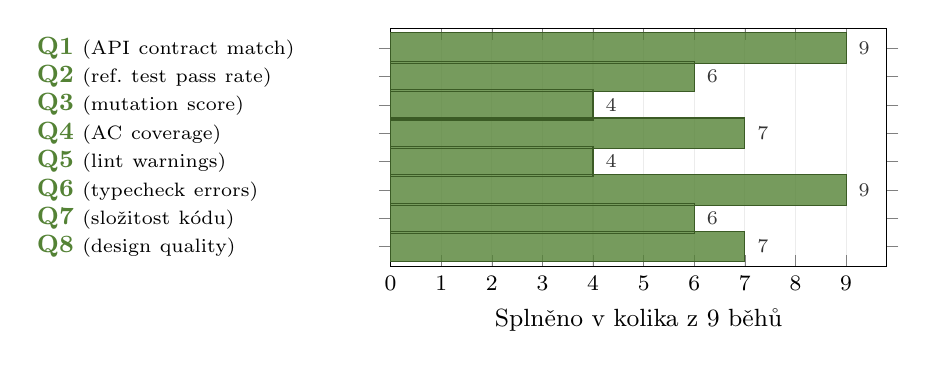
\begin{tikzpicture}
\begin{axis}[
    xbar,
    width=0.65\textwidth,
    height=0.38\textwidth,
    xlabel={Splněno v~kolika z~9 běhů},
    xmin=0, xmax=9.8,
    xtick={0,1,2,3,4,5,6,7,8,9},
    ymin=0.3, ymax=8.7,
    ytick={1,2,3,4,5,6,7,8},
    yticklabels={
        {\textcolor{cQual}{\textbf{Q8}} {\scriptsize(design quality)}},
        {\textcolor{cQual}{\textbf{Q7}} {\scriptsize(složitost kódu)}},
        {\textcolor{cQual}{\textbf{Q6}} {\scriptsize(typecheck errors)}},
        {\textcolor{cQual}{\textbf{Q5}} {\scriptsize(lint warnings)}},
        {\textcolor{cQual}{\textbf{Q4}} {\scriptsize(AC coverage)}},
        {\textcolor{cQual}{\textbf{Q3}} {\scriptsize(mutation score)}},
        {\textcolor{cQual}{\textbf{Q2}} {\scriptsize(ref.\ test pass rate)}},
        {\textcolor{cQual}{\textbf{Q1}} {\scriptsize(API contract match)}}
    },
    yticklabel style={font=\small, anchor=east, text width=12em, align=left},
    xticklabel style={font=\footnotesize},
    xlabel style={font=\small},
    bar width=11pt,
    nodes near coords,
    nodes near coords style={font=\scriptsize, anchor=west, xshift=1pt},
    xmajorgrids=true,
    ymajorgrids=false,
    grid style={gray!15},
    clip=false,
]

\addplot[fill=cQual, draw=cQual!70!black, fill opacity=0.8] coordinates {
    (7,1)   % Q8 >=2/3: 7/9
    (6,2)   % Q7 <=1: 6/9
    (9,3)   % Q6 =0: 9/9
    (4,4)   % Q5 <=1: 4/9
    (7,5)   % Q4 >=24: 7/9
    (4,6)   % Q3 >=70%: 4/7 (2 N/A)
    (6,7)   % Q2 >=37: 6/9
    (9,8)   % Q1 match: 9/9
};

\end{axis}
\end{tikzpicture}
\caption{Míra splnění exit kritérií \mgrp{Q} napříč devíti běhy.
\acs{Q1} a~\acs{Q6} byly splněny ve všech bězích;
\acs{Q3} a~\acs{Q5} nejméně často.
\acs{Q3} počítáno ze~7 běhů (2~bez dat).
Metriky efektivity (E1--E3) nemají exit kritérium a~nejsou zahrnuty.}
\label{fig:variability-quality}
\end{figure}


\definecolor{cQual}{HTML}{548235}

\begin{figure}[H]
\centering
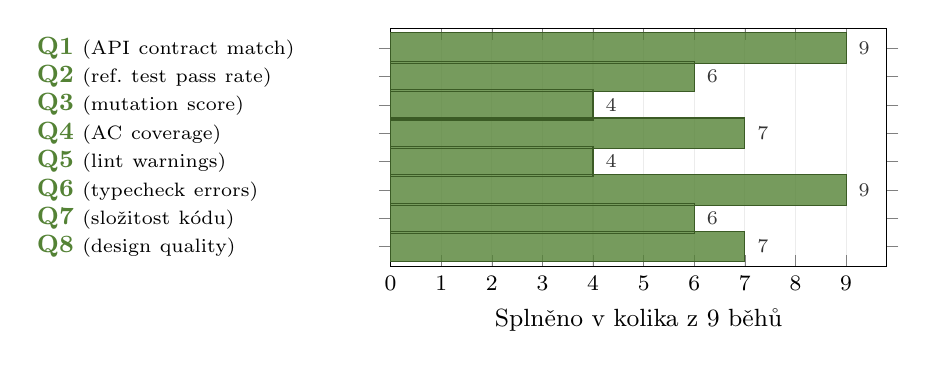
\begin{tikzpicture}
\begin{axis}[
    xbar,
    width=0.65\textwidth,
    height=0.38\textwidth,
    xlabel={Splněno v~kolika z~9 běhů},
    xmin=0, xmax=9.8,
    xtick={0,1,2,3,4,5,6,7,8,9},
    ymin=0.3, ymax=8.7,
    ytick={1,2,3,4,5,6,7,8},
    yticklabels={
        {\textcolor{cQual}{\textbf{Q8}} {\scriptsize(design quality)}},
        {\textcolor{cQual}{\textbf{Q7}} {\scriptsize(složitost kódu)}},
        {\textcolor{cQual}{\textbf{Q6}} {\scriptsize(typecheck errors)}},
        {\textcolor{cQual}{\textbf{Q5}} {\scriptsize(lint warnings)}},
        {\textcolor{cQual}{\textbf{Q4}} {\scriptsize(AC coverage)}},
        {\textcolor{cQual}{\textbf{Q3}} {\scriptsize(mutation score)}},
        {\textcolor{cQual}{\textbf{Q2}} {\scriptsize(ref.\ test pass rate)}},
        {\textcolor{cQual}{\textbf{Q1}} {\scriptsize(API contract match)}}
    },
    yticklabel style={font=\small, anchor=east, text width=12em, align=left},
    xticklabel style={font=\footnotesize},
    xlabel style={font=\small},
    bar width=11pt,
    nodes near coords,
    nodes near coords style={font=\scriptsize, anchor=west, xshift=1pt},
    xmajorgrids=true,
    ymajorgrids=false,
    grid style={gray!15},
    clip=false,
]

\addplot[fill=cQual, draw=cQual!70!black, fill opacity=0.8] coordinates {
    (7,1)   % Q8 >=2/3: 7/9
    (6,2)   % Q7 <=1: 6/9
    (9,3)   % Q6 =0: 9/9
    (4,4)   % Q5 <=1: 4/9
    (7,5)   % Q4 >=24: 7/9
    (4,6)   % Q3 >=70%: 4/7 (2 N/A)
    (6,7)   % Q2 >=37: 6/9
    (9,8)   % Q1 match: 9/9
};

\end{axis}
\end{tikzpicture}
\caption{Míra splnění exit kritérií \mgrp{Q} napříč devíti běhy.
\acs{Q1} a~\acs{Q6} byly splněny ve všech bězích;
\acs{Q3} a~\acs{Q5} nejméně často.
\acs{Q3} počítáno ze~7 běhů (2~bez dat).
Metriky efektivity (E1--E3) nemají exit kritérium a~nejsou zahrnuty.}
\label{fig:variability-quality}
\end{figure}
